\section{数值仿真与分析}
\label{sec:numerical}


\subsection{仿真设置}
为验证上述分析，选取两个二维耦合系统，分别考察损伤组成、双预算下的可达到损伤和记录观察时域的影响。
两组状态矩阵取为
\begin{equation}
 {\bm{A}}_{\rm S}=\begin{bmatrix}0.82&0.18\\-0.10&0.72\end{bmatrix},\qquad
 {\bm{A}}_{\rm U}=\begin{bmatrix}1.04&0.12\\0.03&0.91\end{bmatrix}.
\end{equation}
两者的谱半径分别约为 $0.7800$ 和 $1.0635$，分别记为稳定工况S和不稳定工况U，均在同一有限时刻评价损伤。
共同参数设置如下：
\begin{equation}
 \begin{gathered}
 {\bm{P}}_0=\begin{bmatrix}0.8&0.12\\0.12&0.6\end{bmatrix},\quad
 {\bm{Q}}=\begin{bmatrix}0.05&0.01\\0.01&0.04\end{bmatrix},\\
 {\bm{R}}=\begin{bmatrix}0.2&0.03\\0.03&0.3\end{bmatrix},\quad
 {\bm{Z}}=\begin{bmatrix}2&0.25\\0.25&1.5\end{bmatrix}.
\end{gathered}
 \label{eq:2d-parameters}
\end{equation}
取 ${\bm{m}}_0=0$、$k=4$、$b_{\rm ref}=0.2$、${\bm{v}}=(1,-1)^\top/\sqrt2$。
其中 $\|\cdot\|_F$ 为Frobenius范数，$\|{\bm{P}}_0{\bm{R}}-{\bm{R}}{\bm{P}}_0\|_F\approx0.02546$，
故两矩阵不能通过同一正交变换同时对角化。
因此，该设置包含矩阵非交换的情形。系统参数和攻击方向均预先固定。
用有理数精确递推可验证，S、U工况中32条 $\gamma_{0:4}$ 历史分别产生32个不同的 ${\bm{P}}_4^+$。
因此在这两组工况中，精确标记与事件串可相互确定，对同一攻击有
$\Delta_{\rm marked}=\Delta_{\rm bits}$，精确标记在本例中没有压缩事件历史的信息量。

采用以下两类因果攻击比较损伤组成。
持续定向策略在 $0,\ldots,k$ 的每次真实发送后注入 $b{\bm{v}}$，使先前载荷修改影响后续触发。
两拍符号策略采用第\ref{sec:bounds}节的等概率正负注入及下一拍补偿，在目标时刻首次攻击。
两者采用相同的系统、欧氏峰值和记录协议，攻击方向及策略未经最优化。
双预算验证则将两拍符号构造给出的合法下界与全策略理论上界比较。

通过完整有限事件树计算总体概率及条件矩，并分别保留各协方差标签。
表\ref{tab:vector-damage}中的TV对应事件串 $\gamma_{0:k+1}$；
完整连续日志的预算可行性则由附录\ref{app:full-kernel}中的解析充分界判定。
以下二维结果均采用普通浮点计算，未作严格区间认证。



\subsection{损伤组成与幅值的影响}

取 $b=0.1$，损伤分解结果如表\ref{tab:vector-damage}所示。
持续定向攻击下，两组工况的平均协方差迹均减小。这是由于先前攻击改变了后续触发概率，进而改变各协方差历史的概率权重。
协方差变化的负项抵消了部分偏差损伤，因此仅采用 $\E_\pi\|{\bm{D}}_k\|_2^2$ 会高估本例的真实MSE增量。
两拍符号攻击在目标时刻的发送决定之后首次修改载荷，目标时刻的协方差分布保持不变。
此时协方差变化项为零，损伤完全来自偏差平方项，且 $J_k=L_{\bm{v}}\kappa^2b^2$。


进一步取 $b\in\{0.025,0.05,0.1,0.2\}$，考察损伤随峰值的变化，见图\ref{fig:vector-damage}。
两拍符号策略在S、U中的 $J_k/b^2$ 分别约为 $0.032185$、$0.057380$，
与解析系数一致。持续定向策略在此幅值范围内也呈近似二次变化。
上述结果与引理\ref{lem:gaussian}的损伤分解一致。
这里比较的是固定策略在相同峰值下的损伤；持续定向策略未按同一完整日志TV预算构造，故不据此评价双预算下的攻击优劣。

\begin{ecusttable}
\centering\small
\tabcaption{二维模型在 $b=0.1$ 时的损伤分解}{Decomposition of estimation damage at $b=0.1$ in the two-dimensional systems}
\label{tab:vector-damage}
\begin{tabular}{llrrrr}
\toprule
Case & Attack & $\E_\pi\|{\bm{D}}_k\|_2^2$ & Covariance change & Damage $J_k$ & Event TV\\
\midrule
S & Persistent & 0.0013158 & -0.0000204 & 0.0012953 & 0.0007824 \\
S & Two-step sign & 0.0003219 & 0.0000000 & 0.0003219 & 0.0000688 \\
U & Persistent & 0.0032524 & -0.0001200 & 0.0031323 & 0.0017151 \\
U & Two-step sign & 0.0005738 & 0.0000000 & 0.0005738 & 0.0001723 \\
\bottomrule
\end{tabular}
\par\smallskip{\footnotesize Note: Each entry is independently rounded to seven decimal places; displayed sums may differ in the last digit.}
\end{ecusttable}

\begin{ecustfigure}
\centering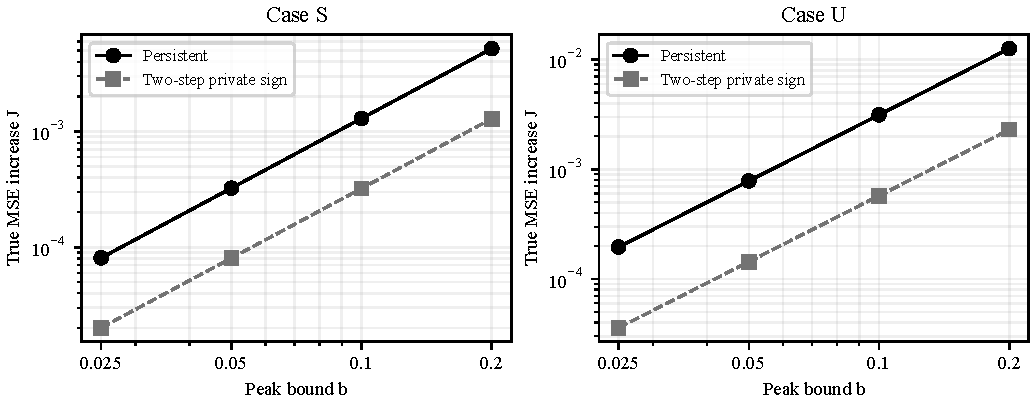
\includegraphics[width=.95\textwidth]{figures/vector_damage.pdf}
\figcaption{两组二维工况的峰值与损伤关系}{Estimation damage versus attack amplitude in the two coupled systems}
\label{fig:vector-damage}
\end{ecustfigure}


\subsection{双预算损伤界的验证}
为同时满足峰值与完整日志TV约束，固定 $b=0.1$，将两拍符号策略以概率
$\lambda=\min\{1,\varepsilon/(C_\pm\kappa^2b^2)\}$ 与无攻击策略混合。
该混合概率由完整日志TV的解析充分界选取，所得策略的损伤由式\eqref{eq:attainable}给出。
相同预算下的损伤上下界如图\ref{fig:vector-budget}所示，计算所用常数见附录\ref{app:validation}。


图中下曲线为合法攻击构造下界，上曲线为幅值界与记录界的较小值：
\[\min\{C_{\rm peak}b^2,C_{\rm record}\varepsilon\}.\]
由图可见，上下界均先随TV预算线性增加，随后达到峰值约束决定的平台，但切换点与比例常数不同。
这一变化对应定理\ref{thm:main}中的两种限制：预算较小时，损伤主要受记录约束限制；预算放宽后，峰值约束起主要作用。
在线性区间内，S、U的上界与合法攻击构造下界之比分别约为783.64和359.14。
因此，上下界在阶数上匹配，其数值常数仍较保守。
按精确协方差标签分别选取偏差半径和统计损伤证书系数，可有限减小记录界常数；
本次选取使两工况的常数最多分别下降约3.25\%和11.99\%，仍未消除这一间隙，见附录\ref{app:label-refinement}。
图中的预算可行性由完整日志联合核的解析界保证。
表\ref{tab:vector-damage}所列事件串TV仅对应较少的信息，不用于替代完整日志约束。


为检查事件树递推的数值实现，两组模型和两类策略的每种组合均进行了40万次独立重置的状态过程模拟。
四项事件树损伤均位于配对模拟的近似95\%置信区间内，最大标准化差异约为1.125。
模型积分、模拟设置及原始结果见附录\ref{app:validation}。
状态过程模拟与事件树结果相符，支持上述数值实现；一般维数的结论由第\ref{sec:bounds}节的理论分析给出。
\begin{ecustfigure}
\centering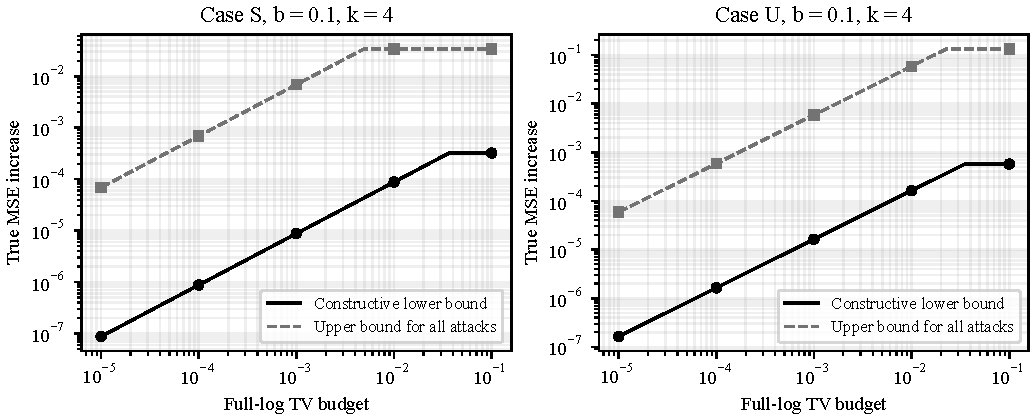
\includegraphics[width=.95\textwidth]{figures/vector_budget.pdf}
\figcaption{合法攻击构造下界与全策略理论上界（$b=0.1$，$k=4$）}{Lower bound from an admissible attack construction and all-policy theoretical upper bound ($b=0.1$, $k=4$)}
\label{fig:vector-budget}
\end{ecustfigure}
\subsection{记录观察时域的影响}
\label{sec:record-ablation}
为考察增加下一事件的作用，在同一攻击策略下改变记录观察时域。沿用S、U系统和目标时刻 $k=4$，
在目标之前不施加攻击，仅在目标发送时实施命题\ref{prop:deletion}的一步保分布MH修改，
之后不再攻击。其提议步长为 $\pm b{\bm{v}}$，拒绝时保持原载荷，故逐路径满足同一峰值限制。
详细平衡使截至目标时刻的完整日志 $H_k$ 与无攻击运行严格同律；
这一等式由解析构造保证。

该策略的损伤、统计损伤证书及记录分布差异如图\ref{fig:record-ablation}所示。
当 $b=0.1$ 时，S、U中的损伤分别约为 $2.995\times10^{-4}$ 和 $5.360\times10^{-4}$，
而扩展事件串 $\gamma_{0:k+1}$ 的TV分别约为 $6.401\times10^{-5}$ 和 $1.609\times10^{-4}$。
加权下一静默事件给出的统计损伤证书分别约为 $4.258\times10^{-4}$ 和 $8.430\times10^{-4}$。
可见，截至目标时刻的日志同律仍伴随正损伤；记录增加下一事件后，预测偏差使静默概率发生变化，从而得到损伤上界。
这里的证书与真实损伤之差反映该固定策略下的保守性，与图\ref{fig:vector-budget}中的全策略最坏损伤界属于不同的比较。

本例各历史下的下一静默概率变化同号，末事件位TV恰等于扩展事件串TV。
该工况据此验证了延长观察时域的作用，但没有体现历史标记相对于末事件位的优势。
历史信息缺失时可能出现的概率抵消由命题\ref{prop:last-bit}给出。
图中统计损伤证书采用总体概率，不含有限样本余量；有限样本置信上界见附录\ref{app:statistical}。
事件串TV也仅为完整扩展日志TV的下界。
接受质量积分、误差诊断及复现步骤见附录\ref{app:record-ablation}。

\begin{ecustfigure}
\centering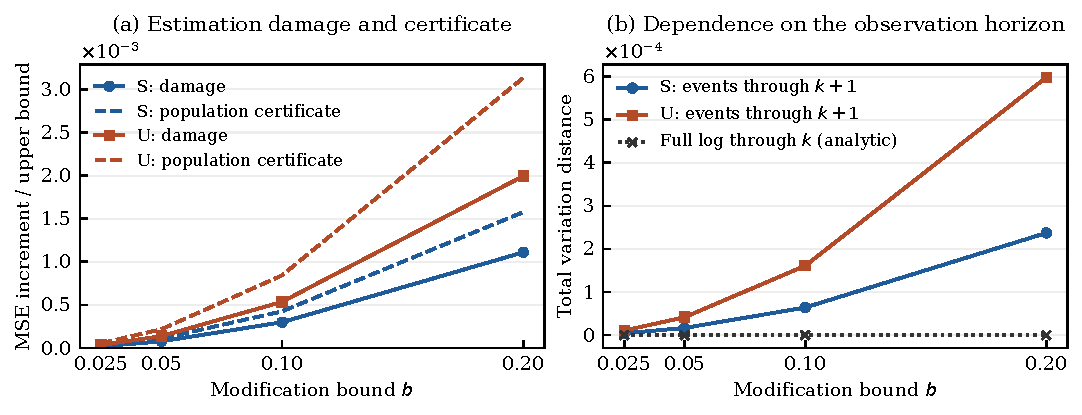
\includegraphics[width=.96\textwidth]{figures/record_conditions.pdf}
\figcaption{同一当拍保分布攻击下的损伤与记录时域对照：截止日志TV为解析零值，扩展事件TV为浮点求积结果}{Damage and record horizons under the same distribution-preserving attack: cutoff-log TV is analytically zero; extended-event TV is evaluated by floating-point quadrature}
\label{fig:record-ablation}
\end{ecustfigure}


\FloatBarrier
